\documentclass{standalone}[9pt]
% main document, called main.tex
\usepackage{tikz}
\usetikzlibrary{external}
\tikzexternalize % activate!
\begin{document}

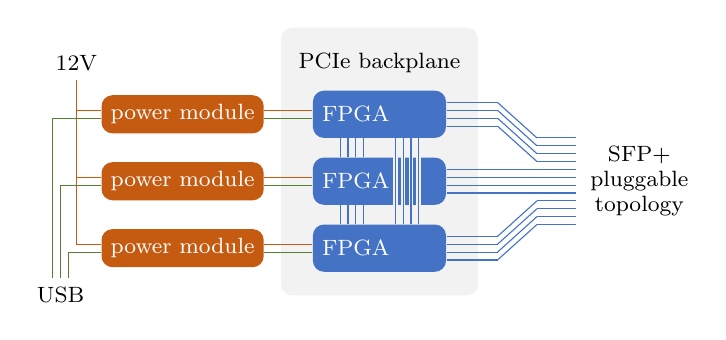
\begin{tikzpicture}
  [scale=.5,auto=left,every node/.style={rectangle,rounded
     corners,fill=myblue,text=white},align=center]
  \definecolor{myblue}{RGB}{68,114,196}
  \definecolor{myorange}{RGB}{197,90,17}
  \definecolor{myorange}{RGB}{197,90,17}
  \definecolor{mygreen}{RGB}{84,130,53}

  \node[fill=gray!10,minimum width=2.5cm,minimum height=3.4cm] (pcie)
     at (0,2.2) {};

  \node[fill=none,text=black] (pcie-label)
     at (0,4.7) {\footnotesize{PCIe backplane}};

%  \node[fill=none,text=black] (pcie0-label) at (0,-1.5) {\footnotesize{PCIe backplane}};

  \node[minimum height=6mm] (fpga0) at (0,0) {\footnotesize{FPGA}\hspace{6mm}};
  \node[minimum height=6mm] (fpga1) at (0,1.7)
    {\footnotesize{FPGA}\hspace{6mm}};
  \node[minimum height=6mm] (fpga2) at (0,3.4)
    {\footnotesize{FPGA}\hspace{6mm}};

  \node[fill=myorange] (power0) at (-5,0) {\footnotesize{power module}};
  \node[fill=myorange] (power1) at (-5,1.7) {\footnotesize{power module}};
  \node[fill=myorange] (power2) at (-5,3.4) {\footnotesize{power module}};

  \draw[arrows=-,>=stealth,color=myorange]
    ([yshift=1mm]power0.east) to ([yshift=1mm]fpga0.west);
  \draw[arrows=-,>=stealth,color=myorange]
    ([yshift=1mm]power1.east) to ([yshift=1mm]fpga1.west);
  \draw[arrows=-,>=stealth,color=myorange]
    ([yshift=1mm]power2.east) to ([yshift=1mm]fpga2.west);

  \draw[arrows=-,>=stealth,color=mygreen]
    ([yshift=-1mm]power0.east) to ([yshift=-1mm]fpga0.west);
  \draw[arrows=-,>=stealth,color=mygreen]
    ([yshift=-1mm]power1.east) to ([yshift=-1mm]fpga1.west);
  \draw[arrows=-,>=stealth,color=mygreen]
    ([yshift=-1mm]power2.east) to ([yshift=-1mm]fpga2.west);

  \draw[arrows=-,>=stealth,color=myblue] ([xshift=-4mm]fpga0.north) to
    ([xshift=-4mm]fpga1.south);
  \draw[arrows=-,>=stealth,color=myblue] ([xshift=-6mm]fpga0.north) to
    ([xshift=-6mm]fpga1.south);
  \draw[arrows=-,>=stealth,color=myblue] ([xshift=-8mm]fpga0.north) to
    ([xshift=-8mm]fpga1.south);
  \draw[arrows=-,>=stealth,color=myblue] ([xshift=-10mm]fpga0.north) to
    ([xshift=-10mm]fpga1.south);
 
   \draw[arrows=-,>=stealth,color=myblue] ([xshift=-4mm]fpga1.north) to
    ([xshift=-4mm]fpga2.south);
  \draw[arrows=-,>=stealth,color=myblue] ([xshift=-6mm]fpga1.north) to
    ([xshift=-6mm]fpga2.south);
  \draw[arrows=-,>=stealth,color=myblue] ([xshift=-8mm]fpga1.north) to
    ([xshift=-8mm]fpga2.south);
  \draw[arrows=-,>=stealth,color=myblue] ([xshift=-10mm]fpga1.north) to
    ([xshift=-10mm]fpga2.south);


   \draw[arrows=-,>=stealth,color=gray!10,line width=0.6mm]
    ([xshift=4mm]fpga1.north) to ([xshift=4mm]fpga1.south);
   \draw[arrows=-,>=stealth,color=gray!10,line width=0.6mm]
    ([xshift=6mm]fpga1.north) to ([xshift=6mm]fpga1.south);
   \draw[arrows=-,>=stealth,color=gray!10,line width=0.6mm]
    ([xshift=8mm]fpga1.north) to ([xshift=8mm]fpga1.south);
   \draw[arrows=-,>=stealth,color=gray!10,line width=0.6mm]
    ([xshift=10mm]fpga1.north) to ([xshift=10mm]fpga1.south);

   \draw[arrows=-,>=stealth,color=myblue] ([xshift=4mm]fpga0.north) to
    ([xshift=4mm]fpga2.south);
  \draw[arrows=-,>=stealth,color=myblue] ([xshift=6mm]fpga0.north) to
    ([xshift=6mm]fpga2.south);
  \draw[arrows=-,>=stealth,color=myblue] ([xshift=8mm]fpga0.north) to
    ([xshift=8mm]fpga2.south);
  \draw[arrows=-,>=stealth,color=myblue] ([xshift=10mm]fpga0.north) to
    ([xshift=10mm]fpga2.south);

  \coordinate (sfp0) at (3,0) {};

  \draw[arrows=-,>=stealth,color=myblue]
    ([yshift=-1mm]fpga0.east) to ([yshift=-1mm]sfp0.west);
  \draw[arrows=-,>=stealth,color=myblue]
    ([yshift=1mm]fpga0.east) to ([yshift=1mm]sfp0.west);
  \draw[arrows=-,>=stealth,color=myblue]
    ([yshift=-3mm]fpga0.east) to ([yshift=-3mm]sfp0.west);
  \draw[arrows=-,>=stealth,color=myblue]
    ([yshift=3mm]fpga0.east) to ([yshift=3mm]sfp0.west);

  \coordinate (sfp1) at (3,1.7) {};

  \draw[arrows=-,>=stealth,color=myblue]
    ([yshift=-1mm]fpga1.east) to ([yshift=-1mm]sfp1.west);
  \draw[arrows=-,>=stealth,color=myblue]
    ([yshift=1mm]fpga1.east) to ([yshift=1mm]sfp1.west);
  \draw[arrows=-,>=stealth,color=myblue]
    ([yshift=-3mm]fpga1.east) to ([yshift=-3mm]sfp1.west);
  \draw[arrows=-,>=stealth,color=myblue]
    ([yshift=3mm]fpga1.east) to ([yshift=3mm]sfp1.west);

  \coordinate (sfp2) at (3,3.4) {};

  \draw[arrows=-,>=stealth,color=myblue]
    ([yshift=-1mm]fpga2.east) to ([yshift=-1mm]sfp2.west);
  \draw[arrows=-,>=stealth,color=myblue]
    ([yshift=1mm]fpga2.east) to ([yshift=1mm]sfp2.west);
  \draw[arrows=-,>=stealth,color=myblue]
    ([yshift=-3mm]fpga2.east) to ([yshift=-3mm]sfp2.west);
  \draw[arrows=-,>=stealth,color=myblue]
    ([yshift=3mm]fpga2.east) to ([yshift=3mm]sfp2.west);

  \coordinate (sfpL) at (4,1.7) {};
  \coordinate (sfpR) at (5,1.7) {};
  \draw[arrows=-,>=stealth,color=myblue]
    ([yshift=1mm]sfpL.east) to ([yshift=1mm]sfpR.west);
  \draw[arrows=-,>=stealth,color=myblue]
    ([yshift=3mm]sfpL.east) to ([yshift=3mm]sfpR.west);
  \draw[arrows=-,>=stealth,color=myblue]
    ([yshift=5mm]sfpL.east) to ([yshift=5mm]sfpR.west);
  \draw[arrows=-,>=stealth,color=myblue]
    ([yshift=7mm]sfpL.east) to ([yshift=7mm]sfpR.west);
  \draw[arrows=-,>=stealth,color=myblue]
    ([yshift=9mm]sfpL.east) to ([yshift=9mm]sfpR.west);
  \draw[arrows=-,>=stealth,color=myblue]
    ([yshift=11mm]sfpL.east) to ([yshift=11mm]sfpR.west);
  \draw[arrows=-,>=stealth,color=myblue]
    ([yshift=-1mm]sfpL.east) to ([yshift=-1mm]sfpR.west);
  \draw[arrows=-,>=stealth,color=myblue]
    ([yshift=-3mm]sfpL.east) to ([yshift=-3mm]sfpR.west);
  \draw[arrows=-,>=stealth,color=myblue]
    ([yshift=-5mm]sfpL.east) to ([yshift=-5mm]sfpR.west);
  \draw[arrows=-,>=stealth,color=myblue]
    ([yshift=-7mm]sfpL.east) to ([yshift=-7mm]sfpR.west);
  \draw[arrows=-,>=stealth,color=myblue]
    ([yshift=-9mm]sfpL.east) to ([yshift=-9mm]sfpR.west);
  \draw[arrows=-,>=stealth,color=myblue]
    ([yshift=-11mm]sfpL.east) to ([yshift=-11mm]sfpR.west);


  \draw[arrows=-,>=stealth,color=myblue]
    ([yshift=-3mm]sfp0.east) to ([yshift=-11mm]sfpL.west);
  \draw[arrows=-,>=stealth,color=myblue]
    ([yshift=-1mm]sfp0.east) to ([yshift=-9mm]sfpL.west);
  \draw[arrows=-,>=stealth,color=myblue]
    ([yshift=1mm]sfp0.east) to ([yshift=-7mm]sfpL.west);
  \draw[arrows=-,>=stealth,color=myblue]
    ([yshift=3mm]sfp0.east) to ([yshift=-5mm]sfpL.west);

  \draw[arrows=-,>=stealth,color=myblue]
    ([yshift=-3mm]sfp2.east) to ([yshift=5mm]sfpL.west);
  \draw[arrows=-,>=stealth,color=myblue]
    ([yshift=-1mm]sfp2.east) to ([yshift=7mm]sfpL.west);
  \draw[arrows=-,>=stealth,color=myblue]
    ([yshift=1mm]sfp2.east) to ([yshift=9mm]sfpL.west);
  \draw[arrows=-,>=stealth,color=myblue]
    ([yshift=3mm]sfp2.east) to ([yshift=11mm]sfpL.west);

  \draw[arrows=-,>=stealth,color=myblue]
    ([yshift=-3mm]sfp1.east) to ([yshift=-3mm]sfpL.west);
  \draw[arrows=-,>=stealth,color=myblue]
    ([yshift=-1mm]sfp1.east) to ([yshift=-1mm]sfpL.west);
  \draw[arrows=-,>=stealth,color=myblue]
    ([yshift=1mm]sfp1.east) to ([yshift=1mm]sfpL.west);
  \draw[arrows=-,>=stealth,color=myblue]
    ([yshift=3mm]sfp1.east) to ([yshift=3mm]sfpL.west);

  \node[text=black,fill=none] (plug) at (6.6,1.7)
    {\footnotesize{SFP+}\\[-1mm]\footnotesize{pluggable}\\[-1mm]
      \footnotesize{topology}};

  \node[fill=none,text=black] (psrc) at (-7.7,4.7)
    {\footnotesize{12V}};
  \coordinate (p2) at (-7.7, 3.4) {};
  \coordinate (p1) at (-7.7, 1.7) {};
  \coordinate (p0) at (-7.7, 0) {};
  \draw[arrows=-,>=stealth,color=myorange]
    ([xshift=0mm]psrc.south) to ([xshift=0mm,yshift=1mm]p0.north);
  \draw[arrows=-,>=stealth,color=myorange]
    ([xshift=0mm,yshift=1mm]p0) to ([yshift=1mm]power0.west);
  \draw[arrows=-,>=stealth,color=myorange]
    ([xshift=0mm,yshift=1mm]p1) to ([yshift=1mm]power1.west);
  \draw[arrows=-,>=stealth,color=myorange]
    ([xshift=0mm,yshift=1mm]p2) to ([yshift=1mm]power2.west);

  \node[fill=none,text=black] (usrc) at (-8.1,-1.2)
    {\footnotesize{USB}};
  \coordinate (usb0) at (-8.1, 0) {};
  \draw[arrows=-,>=stealth,color=mygreen]
    ([xshift=2mm]usrc.north) to ([xshift=2mm,yshift=-1mm]usb0.south);
  \draw[arrows=-,>=stealth,color=mygreen]
    ([xshift=2mm,yshift=-1mm]usb0) to ([yshift=-1mm]power0.west);

  \coordinate (usb1) at (-8.1, 1.7) {};
  \draw[arrows=-,>=stealth,color=mygreen]
    ([xshift=0mm]usrc.north) to ([xshift=0mm,yshift=-1mm]usb1.south);
  \draw[arrows=-,>=stealth,color=mygreen]
    ([xshift=0mm,yshift=-1mm]usb1) to ([yshift=-1mm]power1.west);

  \coordinate (usb2) at (-8.1, 3.4) {};
  \draw[arrows=-,>=stealth,color=mygreen]
    ([xshift=-2mm]usrc.north) to ([xshift=-2mm,yshift=-1mm]usb2.south);
  \draw[arrows=-,>=stealth,color=mygreen]
    ([xshift=-2mm,yshift=-1mm]usb2) to ([yshift=-1mm]power2.west);
 
\end{tikzpicture}

\end{document}
